\documentclass[10pt, a4paper]{article}

\usepackage[utf8]{inputenc}
\usepackage[portuges]{babel}
\usepackage{blindtext}
\usepackage{enumitem}
\usepackage{graphicx}
\usepackage{cite}

\title{Desenvolvimento de Sistemas de Software \\ \large{Mestrado Integrado em Engenharia Informática}}
\author{Luís Capa \\ A81960 \\ 
\includegraphics[width = 20mm]{luis}
	\and 
	Moisés Antunes \\ A82263 \\ 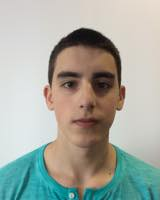
\includegraphics[width = 20mm]{moises}
	\and
	Pedro Capa \\ A83170 \\ 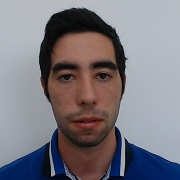
\includegraphics[width = 20mm, height = 25mm]{pedro}
}
\date{\today}

\renewcommand{\baselinestretch}{1.2}

\newpage
\begin{document}
\maketitle
\tableofcontents

\newpage
\section{Introdução}\label{Intro}
Hoje em dia, os clientes das grandes marcas de automóveis têm a possibilidade de personalizar o carro da maneira como quiserem. Para tal, os clientes podem escolher peça a peça, escolher um pacote ou escolher configuração ótima em relação ao orçamento. O cliente não pode escolher todas as peças que quer, visto que há peças que são incompatíveis e outras que são obrigatórias. Os componentes na fábrica têm um stock, no caso de chegarem novas peças é necessário informar o sistema que chegaram novas peças e os carros que estão à espera dessas peças voltam para a fila de produção.
Como este modelo de compra está a ser muito usado, o trabalho de DSS deste ano consistia em modelar o problema, recorrendo à linguagem de modelação UML, para criar a interface gráfica da aplicação e para criar as classes deste projeto, foi recorrido à linguagem de programação Java. O sistema de base de dados utilizado foi o MySQL.


\section{Objetivos}\label{objetivos}
Esta unidade curricular tem o objetivo de mudar a forma como nós programamos, pois até agora sempre que recebiamos um projeto o primeiro pensamento era escrever código. Para isso usou-se a linguagem UML para preparar a escrita do código de forma a cometer menos erros quer na criação de classes e nas suas variáveis de instância quer ter uma representação gráfica do sistema a ser desenvolvido.
Este relatório tem o objetivo de clarificar o trabalho realizado no geral, bem como as suas partes.


\newpage
\section{Trabalho realizado}\label{trabalho}
Para este trabalho foram criados alguns modelos UML como o modelo de dominio, UseCase, os diagramas de estado, os diagramas de sequência, diagramas de classes e os diagramas de packages.


\subsection{Modelo de domínio}
Inicialmente, no "Visual Paradigm" foi criado um modelo de domínio que mostra os principais conceitos e relações entre entidades criadas para este problema, a título de exemplo, foram consideradas algumas relações entre os componentes do carro.
\begin{figure}[!htb]
\centering
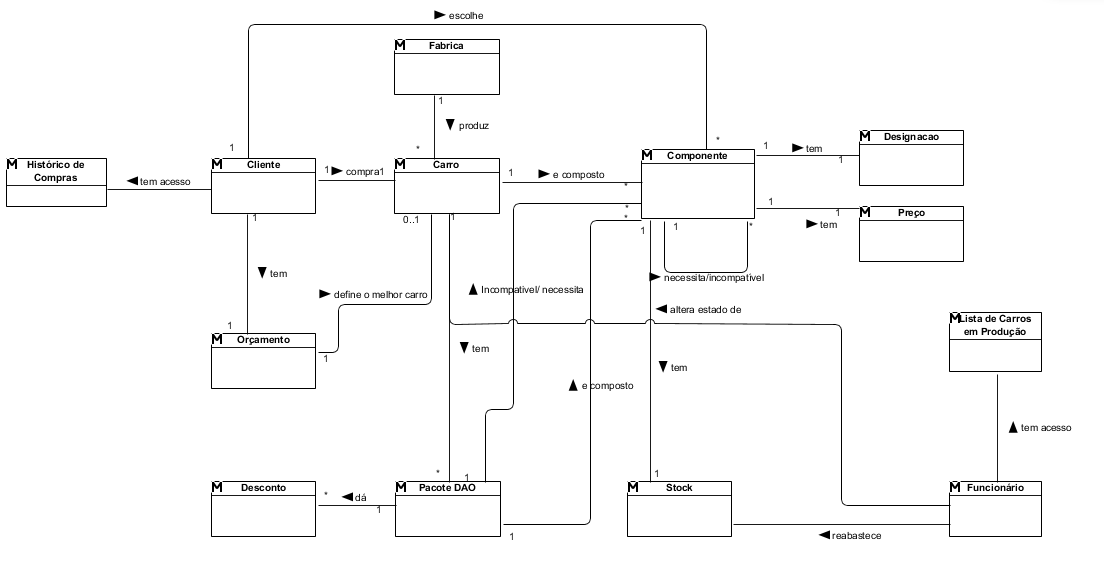
\includegraphics[width=12cm]{Modelo_de_Dominio}
\caption{Modelo de domínio}
\label{MD}
\end{figure}


\subsection{Diagrama de use cases}
De seguida, no mesmo programa foi criado o modelo de use cases. Este modelo mostra as principais interações entre os atores do sistema com o própio sistema.De notar que só foram criados os use cases que achamos absolutamente necessário para cumprir alguns requisitos pré-estabelecidos. Tendo em conta que o use case Comprar Carro iria ficar muito extenso, foi dicidido que era melhor dividi-lo em quatro, o Comprar Carro, Escolher Pacote, Escolher Especificações e o Escolher Configuração Ótima. Para cada use case foi feita uma descrição detalhada da iteração entre o ator e o sistema. Neste sistema foram considerados dois atores, o cliente que faria a compra online e o funcionário que utilizaria a aplicação na fábrica.

\begin{figure}[!htb]
\centering
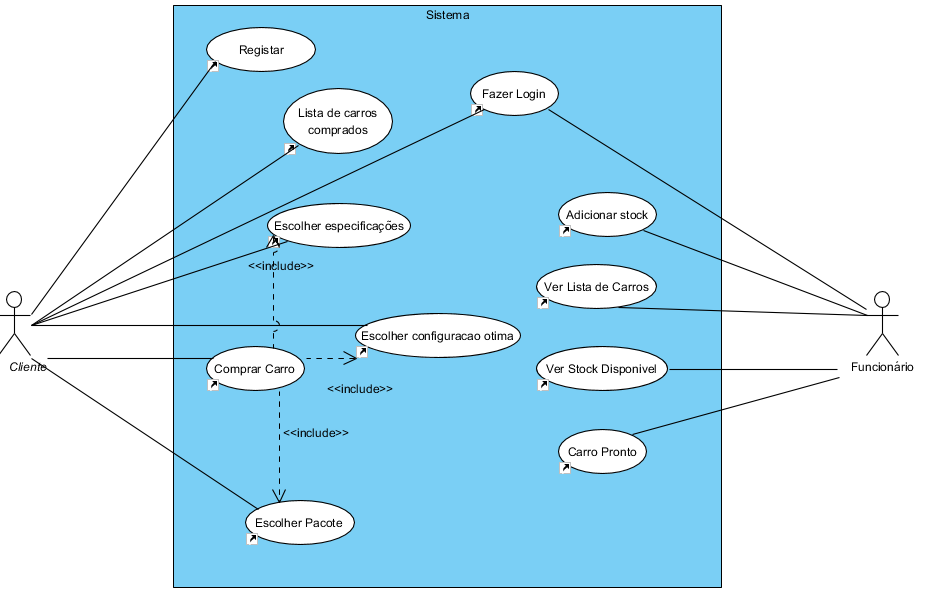
\includegraphics[width=12cm]{Diagrama_UC}
\caption{Diagrama de Use Cases}
\label{Diagrama UC}
\end{figure}


\newpage
\subsection{Especificações de use cases}
Para cada use case, foi criado um modelo no "Excel", que tinha a interação detalhada entre o ator do sistema e o sistema, no qual representava o cenário normal da interação para esse use case, mas também mostrava alternativas e exceções a este. Este também indicavam as pré e pós condições do use case e qual o ator para esse use case em particular. As seguintes imagens são alguns exemplos da especificação de cada use case.

\begin{figure}[!htb]
\centering
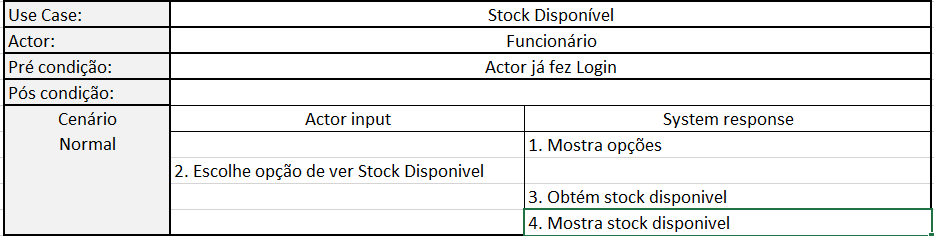
\includegraphics[width=12cm]{ExcelStockDisponivel}
\caption{Descrição do use case Ver Stock Disponvível}
\label{EVSD}
\end{figure}

\begin{figure}[!htb]
\centering
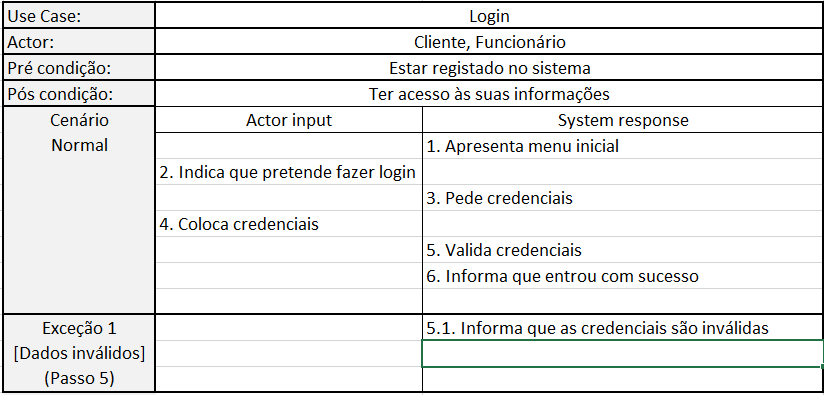
\includegraphics[width=12cm]{ExcelLogin}
\caption{Descrição do use case Login}
\label{EL}
\end{figure}

\begin{figure}[!htb]
\centering
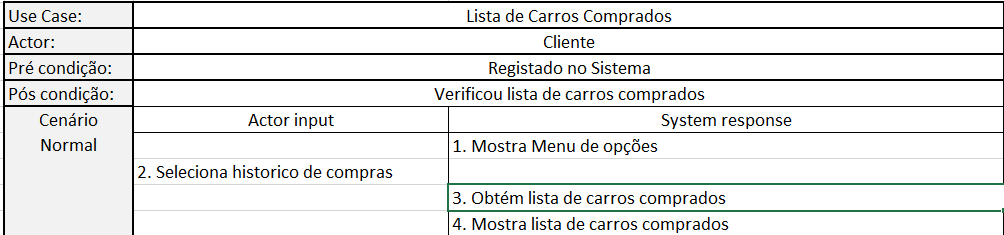
\includegraphics[width=12cm]{ExcelListadeCarrosComprados}
\caption{Descrição do use case Ver Lista de Carros Produção}
\label{EVCP}
\end{figure}

\begin{figure}[!htb]
\centering
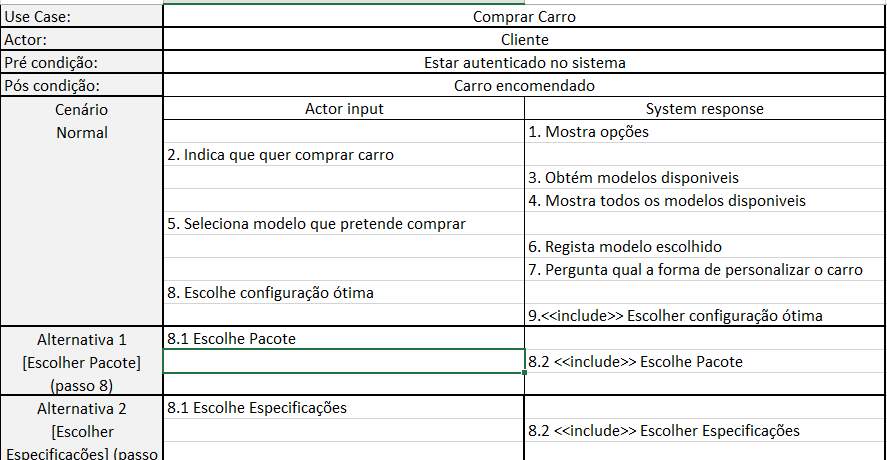
\includegraphics[width=12cm, height=7cm]{ExcelComprarCarro}
\caption{Descrição do use case Comprar Carro, que acaba por se dividir em mais três}
\label{ECC}
\end{figure}


\newpage
\subsection{Protótipo da interface}
Tendo em conta os use cases que foram criados, foi pensado uma forma dos utilizadores interagirem com o sistema. Assim, foram feitas alguns protótipos para cada use case. Sempre que um utilizador realizava uma ação inválida aparecia uma nova janela no ecrã que indicava o motivo do aviso, por exemplo, se um utilizador se tentasse autenticar a aplicação mostrava uma janela que indicava que não se conseguiu autenticar. Quando fazia uma ação válida abria uma nova página e fechava a anterior, exceto se fosse o menu principal.

\begin{figure}[!htb]
\centering
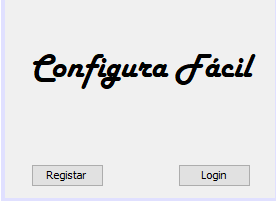
\includegraphics[width=7cm]{InterfaceConfiguraFacil}
\caption{Menu Inicial}
\label{Menu I}
\end{figure}

\begin{figure}[!htb]
\centering
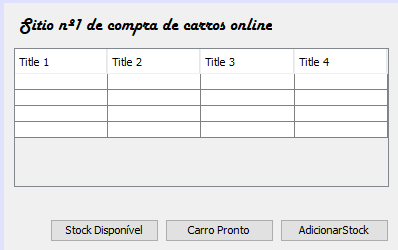
\includegraphics[width=7cm]{InterfaceMenuPrincipalFuncionario}
\caption{Menu principal do funcionário}
\label{Menu PF}
\end{figure}

\begin{figure}[!htb]
\centering
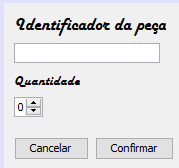
\includegraphics[width=3.5cm]{InterfaceAdicionarStock}
\caption{Janela na qual o funcionário vai adicionar stock}
\label{Menu AS}
\end{figure}

\begin{figure}[!htb]
\centering
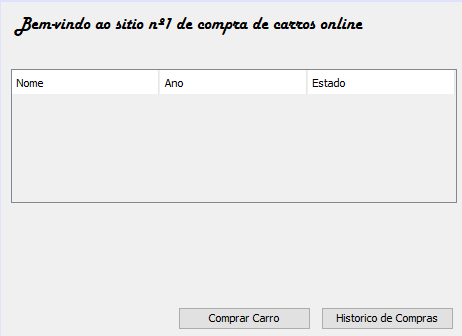
\includegraphics[width=7cm]{InterfaceMenuPrincipal}
\caption{Menu principal do cliente}
\label{Menu CO}
\end{figure}

\begin{figure}[!htb]
\centering
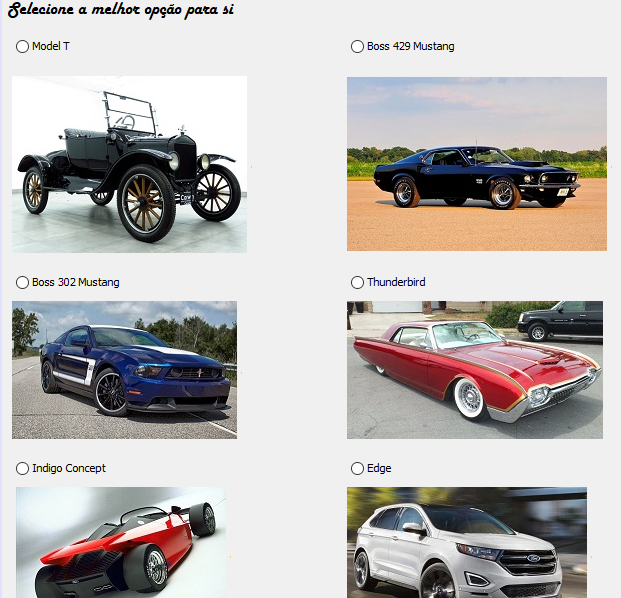
\includegraphics[width=8cm]{InterfaceComprarCarro}
\caption{Menu no qual o cliente vai comprar o carro, começando por escolher o modelo e depois a forma da compra}
\label{Menu CC}
\end{figure}

\newpage
Este sistema não foi totalmente fiável, porque à medida que o trabalho foi desenvolvido estes modelos foram um pouco alterados e ainda foi acrescentado um menu.


\subsection{Máquinas de estado}
No desenvolvimento da aplicação foram consideradas duas entidades que teriam diferentes estados, o carro e a peça. Para descrever as diferentes fases destas entidades foi criado para cada uma um modelo de estado. A figura \ref{ME_Carro} e a figura \ref{ME_Peca}, representam, respetivamente o estado, quer do carro, quer da peça.

\begin{figure}[!htb]
\centering
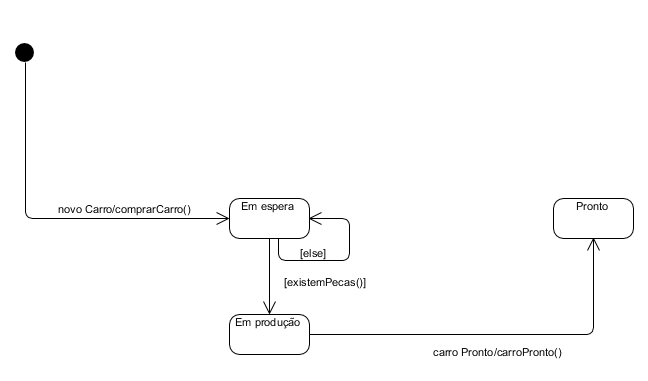
\includegraphics[width=12cm]{MaquinaEstadoCarro}
\caption{Máquina de estados da entidade Carro}
\label{ME_Carro}
\end{figure}

\begin{figure}[!htb]
\centering
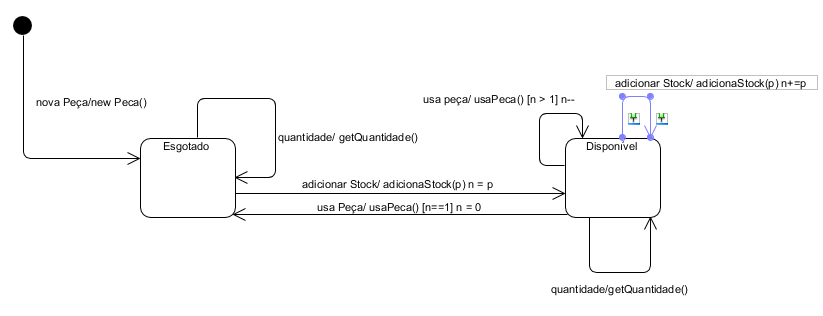
\includegraphics[width=12cm]{MaquinaEstadoPeca}
\caption{Máquina de estados da entidade Peça}
\label{ME_Peca}
\end{figure}


\subsection{Diagrama de sequência de sistemas}
Para se obter uma melhor perceção da interação entre o cliente e o sistema foram criados os diagrama de sequência de sistema para cada use case, baseados nas descrições de cada um, dando uma melhor ideia da interação entre o ator e o sistema. As figuras abaixo, são alguns exemplos de DSS baseados na especificação dos use cases.

\begin{figure}[!htb]
\centering
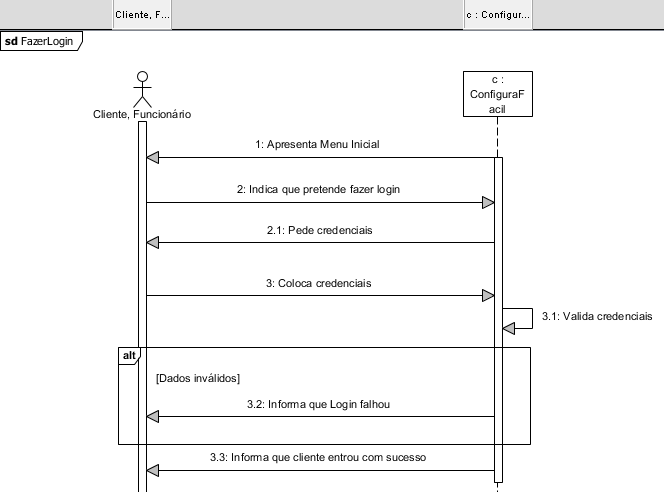
\includegraphics[width=12cm]{FazerLogin}
\caption{DSS do use case Fazer Login}
\label{DSS FL}
\end{figure}

\begin{figure}[!htb]
\centering
\includegraphics[width=12cm]{stockDisponivel}
\caption{DSS do use case Stock Disponível}
\label{DSS SD}
\end{figure}

\begin{figure}[!htb]
\centering
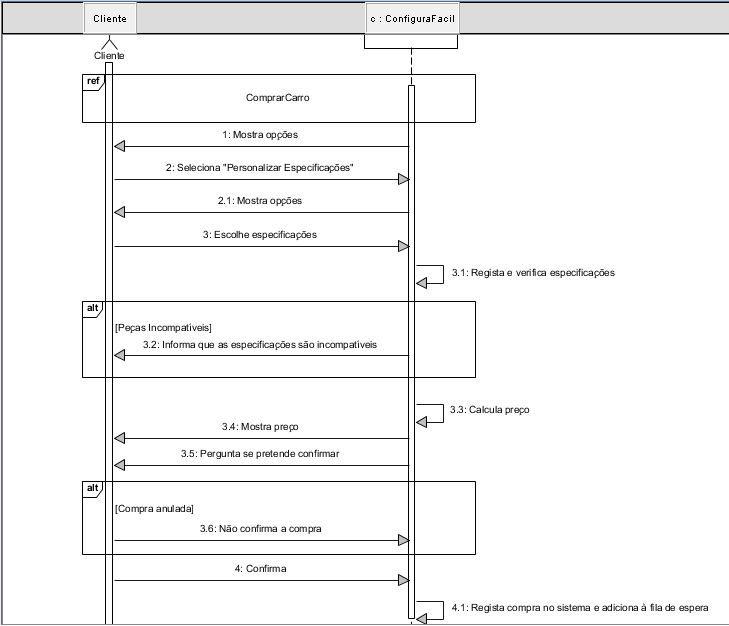
\includegraphics[width=12cm]{EscolherEspecificacoes}
\caption{DSS do use case Escolher Especificações}
\label{DSS EE}
\end{figure}

Em segundo lugar, foram criados os DSS que além de representar a interação do sistema com o utilizador, também representava a relação entre a interface do sistema e a camada de negócio deste. Em sguida foram criados os DSS de subsistemas, que, basicamente, representa as várias entidades no sistema e como cada use case interage com essas entidades, por exemplo o use case "Adicionar Stock" relacionava-se com o subsistema da peça e do carro. 

\begin{figure}[!htb]
\centering
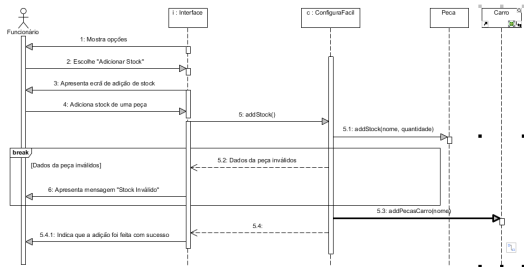
\includegraphics[width=10cm]{DSSSubAddStock}
\caption{DSS de subsistemas do use case Adicionar Stock}
\label{DSSSubAS}
\end{figure}

\begin{figure}[!htb]
\centering
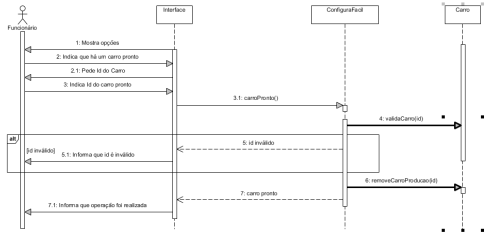
\includegraphics[width=10cm]{DSSSubCarroPronto}
\caption{DSS de subsistemas do use case Carro Pronto}
\label{DSSSubCP}
\end{figure}


\newpage
\subsection{Diagramas de Implementação}
De seguida, foram criados DSS para especificar os métodos que eram utilizados nos DSS anteriores. A partir de alguns dos útlimos DSS, aqueles que tinham de aceder à base de dados, foram criados uns DSS, em que as listas e os conjuntos de entidades eram subsitituídas por DAO, classes que acediam à base de dados, por exemplo no método getListaCarrosComprados(), antes o sistema ia a um map buscar os carros que eram do cliente, mas no último DSS esse map era substituído pela classe CarroDAO, que continha um método para trazer da base de dados as especificações dos carros que o cliente comprou.

\begin{figure}[!htb]
\centering
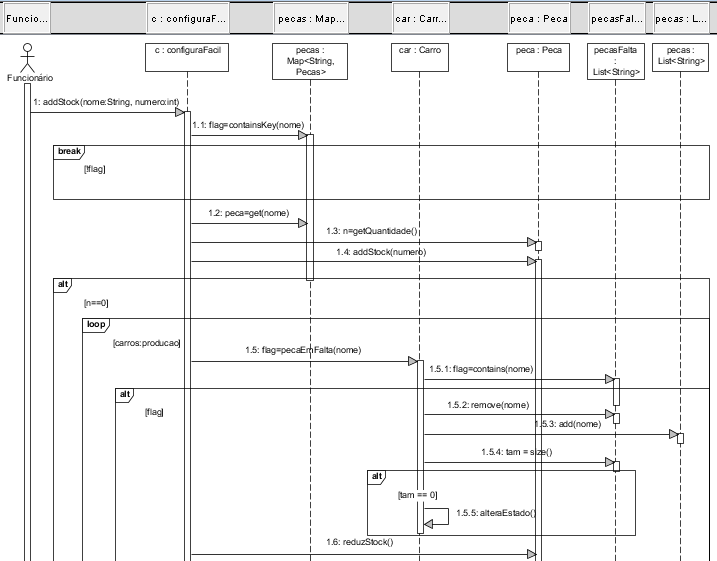
\includegraphics[width=11cm]{DIAddStock}
\caption{Diagrama de Implementação AddStock}
\label{DIAS}
\end{figure}

\begin{figure}[!htb]
\centering
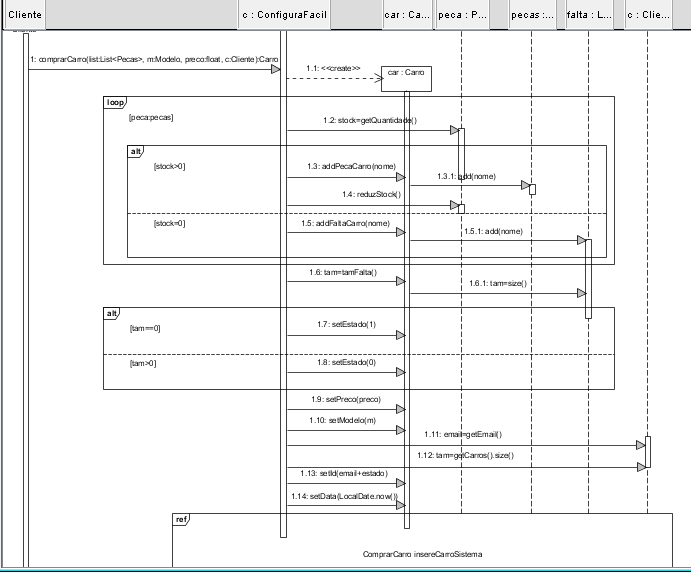
\includegraphics[width=11cm]{DIcomprarCarrocomprarCarro}
\caption{Diagrama de Implementação Comprar Carro}
\label{DICC}
\end{figure}

\begin{figure}[!htb]
\centering
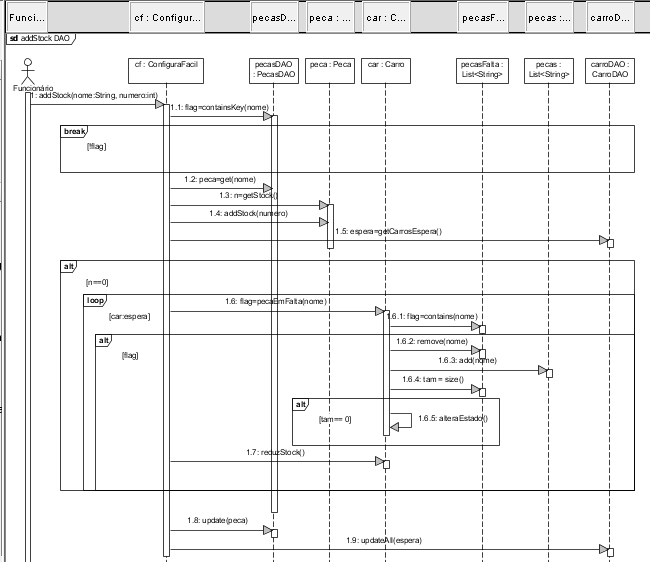
\includegraphics[width=11cm]{DIAddStockDAO}
\caption{Diagrama de Implementação AddStockDAO}
\label{DIASDAO}
\end{figure}

\begin{figure}[!htb]
\centering
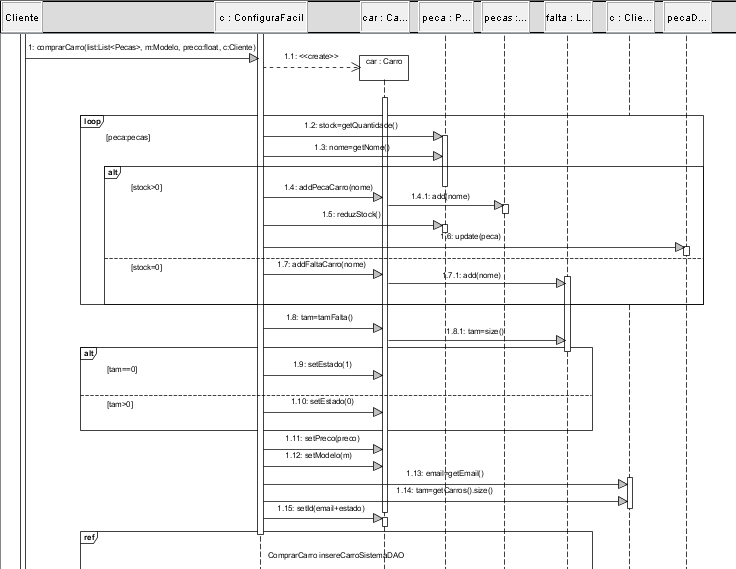
\includegraphics[width=11cm]{DIcomprarCarrocomprarCarroDAO}
\caption{Diagrama de Implementação Comprar Carro DAO}
\label{DICCDAO}
\end{figure}


\newpage
\subsection{Diagrama de classes}
Para os DSS criados foi criado um diagrama de classes, que indicava as classes que eram precisas criar, as variáveis de instância para cada classe e todos os métodos que eram necessários implementar. Não foram criados diagramas de classes para todos os DSS, pois os use cases do "Escolher configuração ótima", "Escolher Especificações" e o "Escolher Pacote" foram todos incluídos no diagrama de classes do "Comprar Carro", pois os métodos nestes DSS eram quase sempre os mesmos e achamos que não havia necessidade de criar diagramas de classes para cada um. O mesmo aconteceu para os diagramas de classes para os DSS que tinham os DAO.
No fim de todos os diagramas de classes serem feitos, foram todos juntados num só, em que continha todas as classes, variáveis de instância e métodos.

\begin{figure}[!htb]
\centering
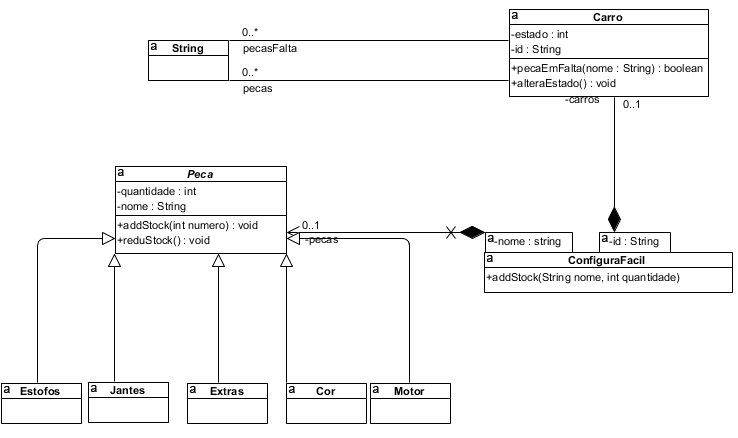
\includegraphics[width=9cm]{DCAdicionarStock}
\caption{Diagrama de classes do use case Adicionar Stock}
\label{DCAS}
\end{figure}

\begin{figure}[!htb]
\centering
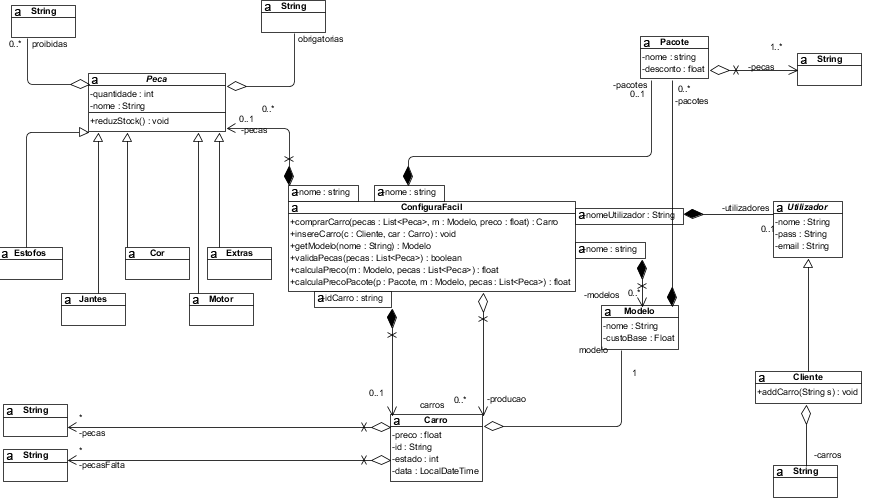
\includegraphics[width=9cm]{DCComprarCarro}
\caption{Diagrama de classes do use case Comprar Carro}
\label{DCCP}
\end{figure}

\begin{figure}[!htb]
\centering
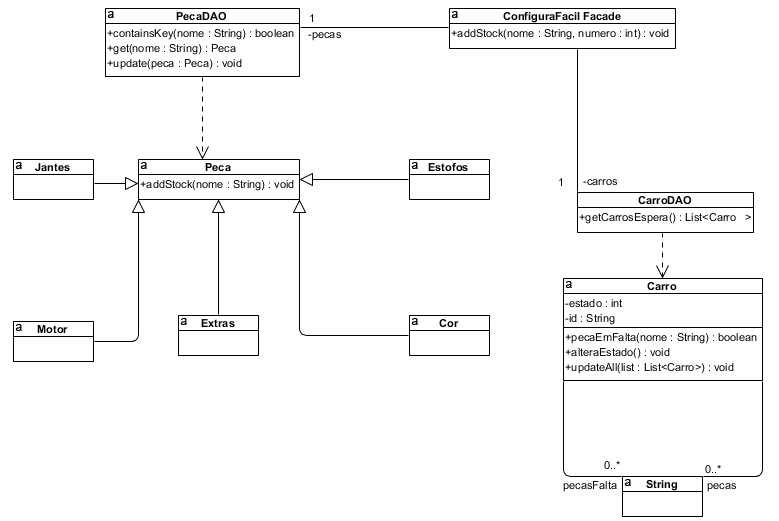
\includegraphics[width=9cm]{DCAdicionarStockDAO}
\caption{Diagrama de classes do use case Adicionar Stock DAO}
\label{DCASDAO}
\end{figure}

\begin{figure}[!htb]
\centering
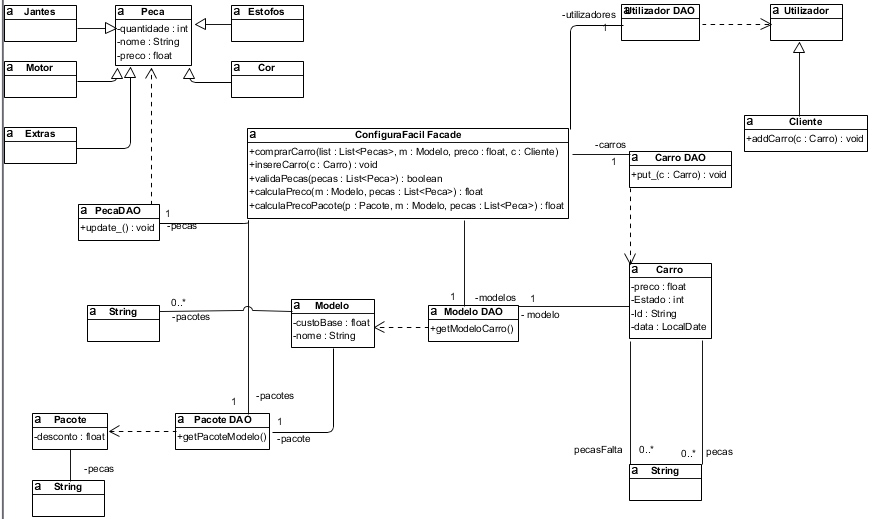
\includegraphics[width=9cm]{DCComprarCarroDAO}
\caption{Diagrama de classes do use case Comprar Carro DAO}
\label{DCCPDAO}
\end{figure}

\begin{figure}[!htb]
\centering
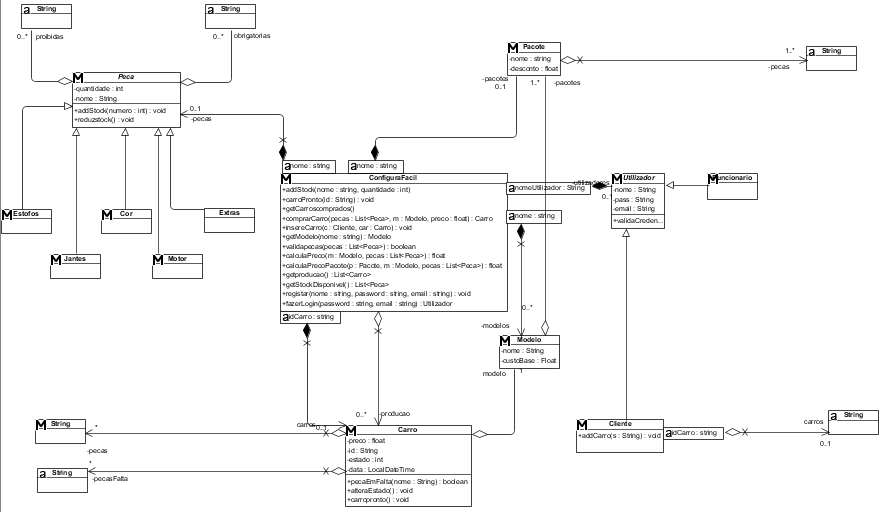
\includegraphics[width=9cm]{DiagramaClasses}
\caption{Diagrama de classes}
\label{DC}
\end{figure}

\begin{figure}[!htb]
\centering
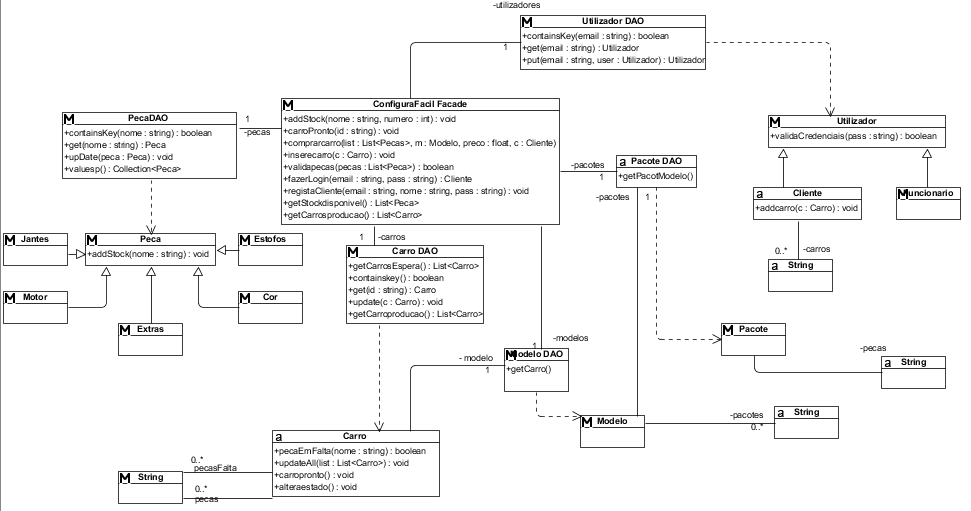
\includegraphics[width=9cm]{DiagramaClassesDAO}
\caption{Diagrama de classes DAO}
\label{DC}
\end{figure}


\newpage
\subsection{Diagrama de packages}
Em seguida, os diagramas de classes e o modelo de domínio foram divididos em packages. Além destes diagramas de packages, do mesmo modo foi criado um diagrama de packages para demonstrar as diferentes camadas aplicacionais do sistema. Esta foi dividida em três partes, a Interface, a camada de negócio e a base de dados. Na camada de negócio estava contida as várias classes do sistema.


\newpage
\section{Funcionamento da aplicação}
Como já foi referido acima há dois tipos de utilizadores, os clientes e os funcionários. Os funcionários são responsáveis por colocar um carro em produção pronto e adicionar peças na fábrica. Quando são adicionadas peças pelos funcionários, o sistema verifica se há algum carro à espera dessa peça e põe essa peça como colocada no carro. O cliente tem acesso à lista de carros que comprou, pode comprar um carro de três formas diferentes, escolher um pacote, escolher a melhor configuração com um determinado orçamento ou personalizar por completo o carro. Na compra do carro, o cliente escolhe primeiro qual o modelo do carro e só em seguida escolhe a forma de compra. Se um cliente escolher um pacote, este não tem a opção de alterar as peças obrigatórias, neste caso, o motor, a cor, jantes e estofos, no entanto, pode escolher todas os extras que quiser. Ao escolher esta opção o cliente tem um desconto associado a cada pacote. Se o cliente escolher personalizar tem a possiblidade de escolher todas as peças que quiser, desde que não tenha peças incompatíveis ou não tenha peças obrigatórias em falta. Ao escolher a configuração ótima não há garantia que tenha a melhor configuração dado o orçamento disponível. Nesta opção o sistema vai tentar encontrar o melhor pacote, ou seja, o pacote mais caro para o dado modelo e orçamento que escolheu. Se ainda houver margem o sistema vai adicionar todos os extras que puder, começando sempre por adicionar os mais caros. Este algoritmo não garante que seja escolhida a melhor configuração, pois não verifica todas as diferentes.


\newpage
\section{Conclusão}\label{analise}
No final, acreditamos que o trabalho que desenvolvemos até agora demonstra bem esse equilíbrio entre personalização e facilidade de uso que procuramos, que são apenas detalhes, mas é neles que se destaca uns projetos dos outros. Também achamos que o essencial foi feito apropriadamente e que não há falta de alguma funcionalidade que seja absolutamente necessário, sendo que consideramos o trabalho até agora tanto funcional como cómodo para o utilizador. Como não tinhamos muita prática em modelação, à medida que o projeto era desenvolvido verificamos que eram cometidos alguns erros na modelação, que nos obrigava a reformular alguns modelos, retardando o desenvolvimento do projeto. Foi notado que se passou menos tempo a corrigir erros no código, mas também foram criados menos métodos e que só foram criados os métodos que eram necessários no desenvolvimento do projeto, comparando com outros projetos, que por vezes eram criados métodos que nunca eram utilizados.
\end{document}